\documentclass[a4paper, 12pt]{article}

%% --- packages --- %%%
\usepackage{subcaption}
%% drawing
\usepackage{tikz}
\usetikzlibrary{
  arrows.meta,
  automata,
  positioning,
  shapes.multipart,
  chains,
  calc,
  math,
  decorations.pathreplacing
} 
%% colors
\usepackage{xcolor}
\definecolor{lightOrange}{rgb}{0.9921875,0.890625,0.69921875}
\definecolor{darkOrange}{rgb}{0.96875,0.64453125,0.33203125}
\definecolor{skyBlue}{rgb}{0.66796875,0.875,0.97265625}
\definecolor{darkBlue}{rgb}{0.046875,0.69140625,0.9375}
%% easier graphs
\usepackage{tkz-graph}
%%% --- end: packages --- %%%

%%% --- commands --- %%%
%% for automata package; create nodes using another node as reference
% 1 - node name
% 2 - inner label
\newcommand{\rtNode}[2]{\node[state] (#1) [label=above: $#1$] {$#2$};}
% 1 - reference node
% 2 - node name, outer label
% 3 - inner label
\newcommand{\rtEA}[3]{\node[state] (#2) [label=above:$#2$, right=of #1] {$#3$};}
\newcommand{\rtWE}[3]{\node[state] (#2) [label=above:$#2$, left=of #1] {$#3$};}
\newcommand{\rtNO}[3]{\node[state] (#2) [label=above:$#2$, above=of #1] {$#3$};}
\newcommand{\rtSO}[3]{\node[state] (#2) [label=above:$#2$, below=of #1] {$#3$};}
\newcommand{\rtNOEA}[3]{\node[state] (#2) [label=above:$#2$, above right=of #1] {$#3$};}
\newcommand{\rtNOWE}[3]{\node[state] (#2) [label=above:$#2$, above left=of #1] {$#3$};}
\newcommand{\rtSOEA}[3]{\node[state] (#2) [label=above:$#2$, below right=of #1] {$#3$};}
\newcommand{\rtSOWE}[3]{\node[state] (#2) [label=above:$#2$, below left=of #1] {$#3$};}
% end: node shortcuts %
% tikz commands for drawing list nodes
% 1 - node name
% 2 - node label
\newcommand{\listNode}[2]{\node[list,on chain] (#1)%
  {\nodepart{second} #2};} 

% 1 - node name
\newcommand{\listHead}[1]{\node[listHead,on chain] (#1) {};} 
\newcommand{\listNil}{\node[listNil,on chain] (nil) {$L. nil$};} 
% end: drawing list nodes %

%% --- global tikz styles --- %%
\tikzset{
  every state/.style={
    fill=lightOrange,
    draw=darkOrange,
    inner sep = 0pt,
    minimum size = 5ex 
  }
}
\tikzset{
  VertexStyle/.style={
    shape        = circle,
    color        = darkOrange,
    fill         = lightOrange,
    inner sep    = 2pt,
    outer sep    = 0pt,
    minimum size = 12pt,
    text         = black,
    draw
  }
}
\tikzset{
  list/.style={
    rectangle split,
    rectangle split parts=3,
    draw,
    rectangle split horizontal,
    minimum size=18,
    inner sep=6pt,
    fill=lightOrange,
    text=black
  }
}
\tikzset{
  listHead/.style={
    rectangle split,
    rectangle split parts=3,
    draw,
    rectangle split horizontal,
    minimum size=18,
    inner sep=5pt,
    fill=skyBlue,
    text=black
  }
}

\tikzset{
  listNil/.style={
    rectangle split,
    rectangle split parts=2,
    rectangle split horizontal,
    minimum size=18,
    inner sep=5pt,
  }
}

%% --- end: global tikz styles --- %%

\begin{document}

\section{Picture-1}
\subsection*{Source}
\begin{figure}[h]
  \centering
  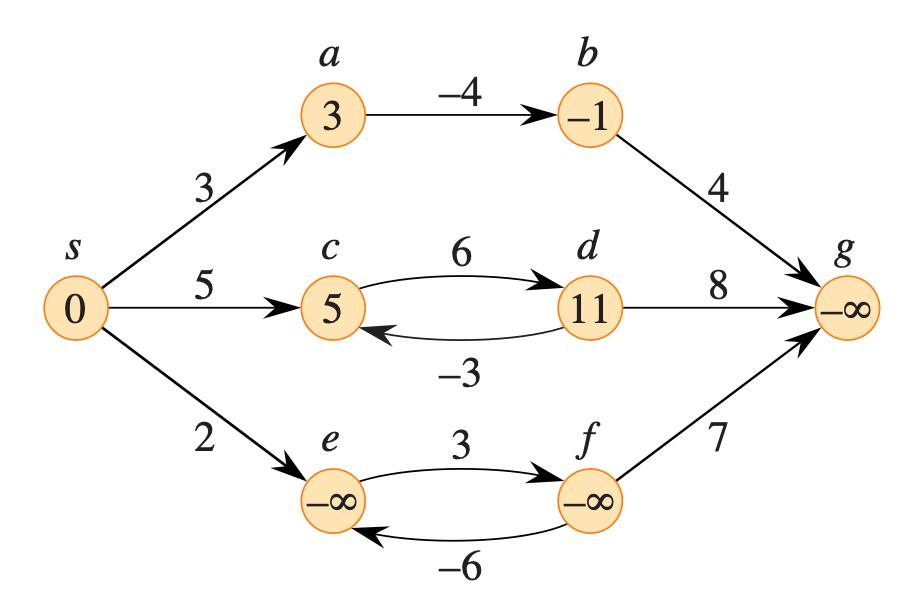
\includegraphics[width=0.7\textwidth]{./src/1.png}
\end{figure}

\subsection*{attempt}
\begin{figure}[h]
  \centering
  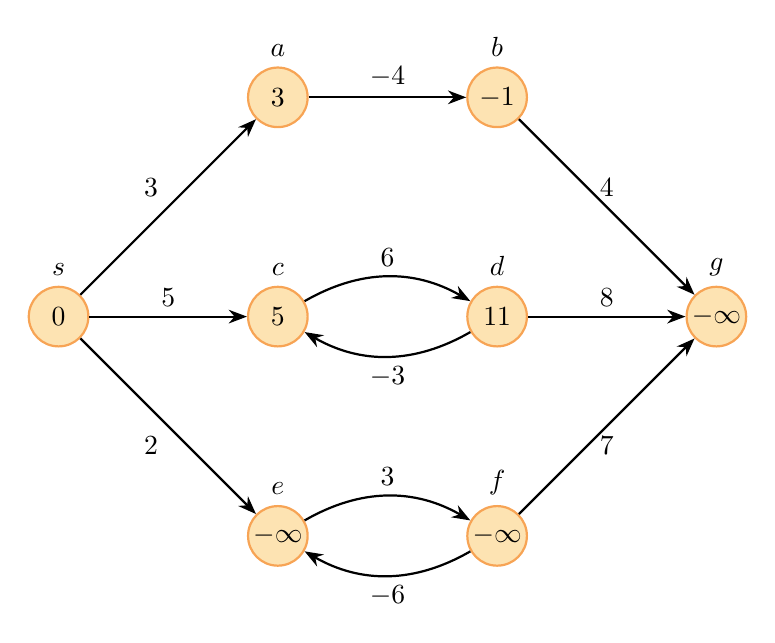
\begin{tikzpicture}[
    >=Stealth,
    node distance=2cm,
    thick
  ]
  \rtNode{s}{0}
  \rtEA{s}{c}{5}
  \rtEA{c}{d}{11}
  \rtEA{d}{g}{-\infty}
  \rtNO{c}{a}{3}
  \rtSO{c}{e}{-\infty}
  \rtNO{d}{b}{-1}
  \rtSO{d}{f}{-\infty}

  \path[->]
  (s) edge              node[above left] {$3$}  (a)
      edge              node[above]      {$5$}  (c)
      edge              node[below left] {$2$}  (e)
  (a) edge              node[above]      {$-4$} (b)
  (c) edge [bend left]  node[above]      {$6$}  (d)
  (d) edge [bend left]  node[below]      {$-3$} (c)
  (e) edge [bend left]  node[above]      {$3$}  (f)
  (f) edge [bend left]  node[below]      {$-6$} (e)
  ;
  \path[<-]
  (g) edge node[above] {$4$} (b)
      edge node[above] {$8$} (d)
      edge node[below] {$7$} (f)
  ;
  \end{tikzpicture}
\end{figure}

\pagebreak
\section{Picture-2}
\subsection*{Source}
\begin{figure}[h]
  \centering
  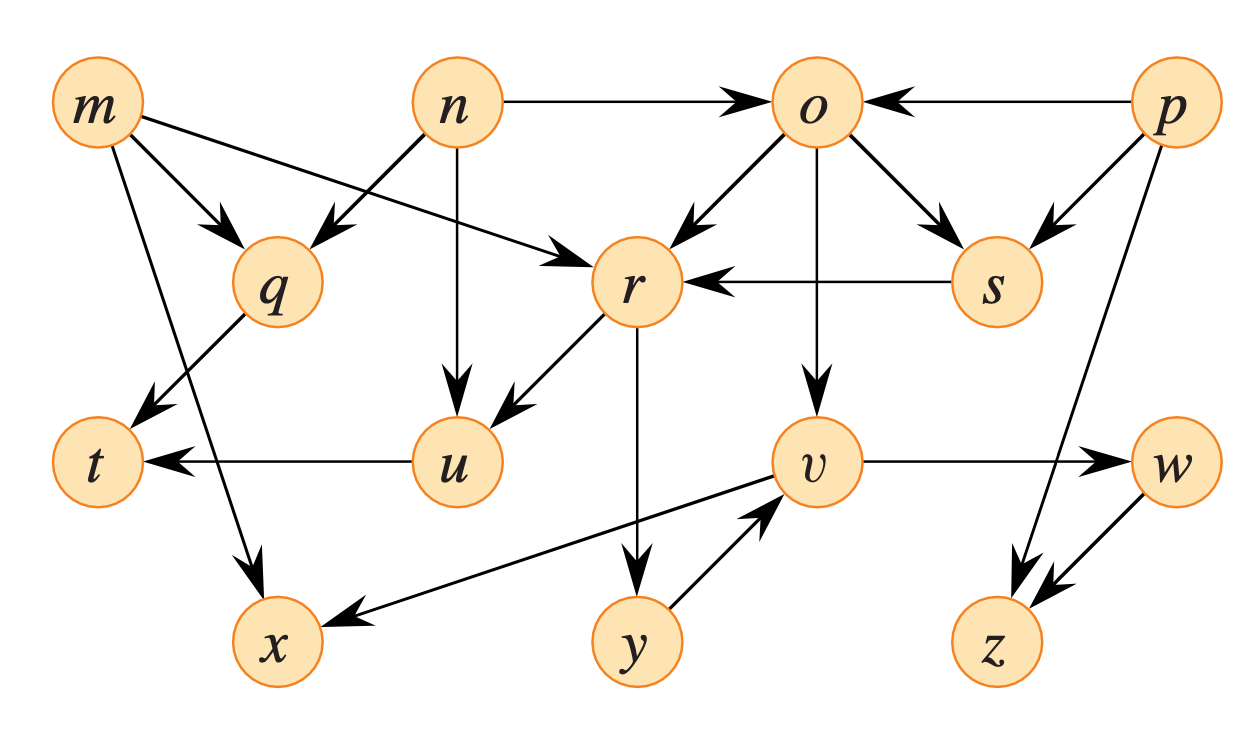
\includegraphics[width=0.7\textwidth]{./src/2.png}
\end{figure}

\subsection*{attempt}
\begin{figure}[h]
  \centering
  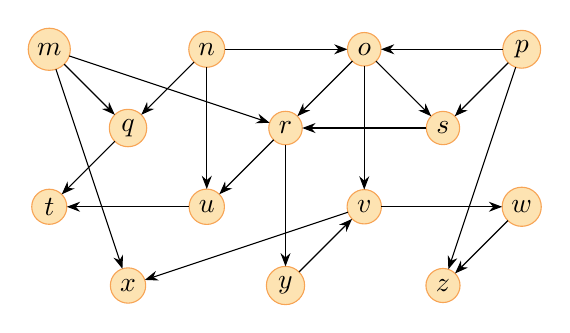
\begin{tikzpicture}[>=Stealth]
    \SetVertexMath

    \Vertex{m}
    \SOEA(m){q}
    \SOWE(q){t}
    \NOEA(q){n}
    \SOEA(q){u}
    \NOEA(u){r}
    \SOEA(u){y}
    \SOWE(u){x}
    \NOEA(r){o}
    \SOEA(r){v}
    \SOEA(o){s}
    \NOEA(s){p}
    \SOEA(s){w}
    \SOWE(w){z}

    \path[->]
    (m) edge (r)
        edge (q)
        edge (x)
    (n) edge (q)
        edge (u)
        edge (o)
    (p) edge (o)
        edge (s)
        edge (z)
    (o) edge (r)
        edge (s)
        edge (v)
    (q) edge (t)
    (s) edge (r)
    (r) edge (u)
        edge (y)
    (u) edge (t)
    (y) edge (v)
    (v) edge (x)
        edge (w)
    (w) edge (z)
        ;
    \end{tikzpicture}
\end{figure}

\pagebreak
\section{Picture-3}
\subsection*{Source}
\begin{figure}[h]
  \centering
  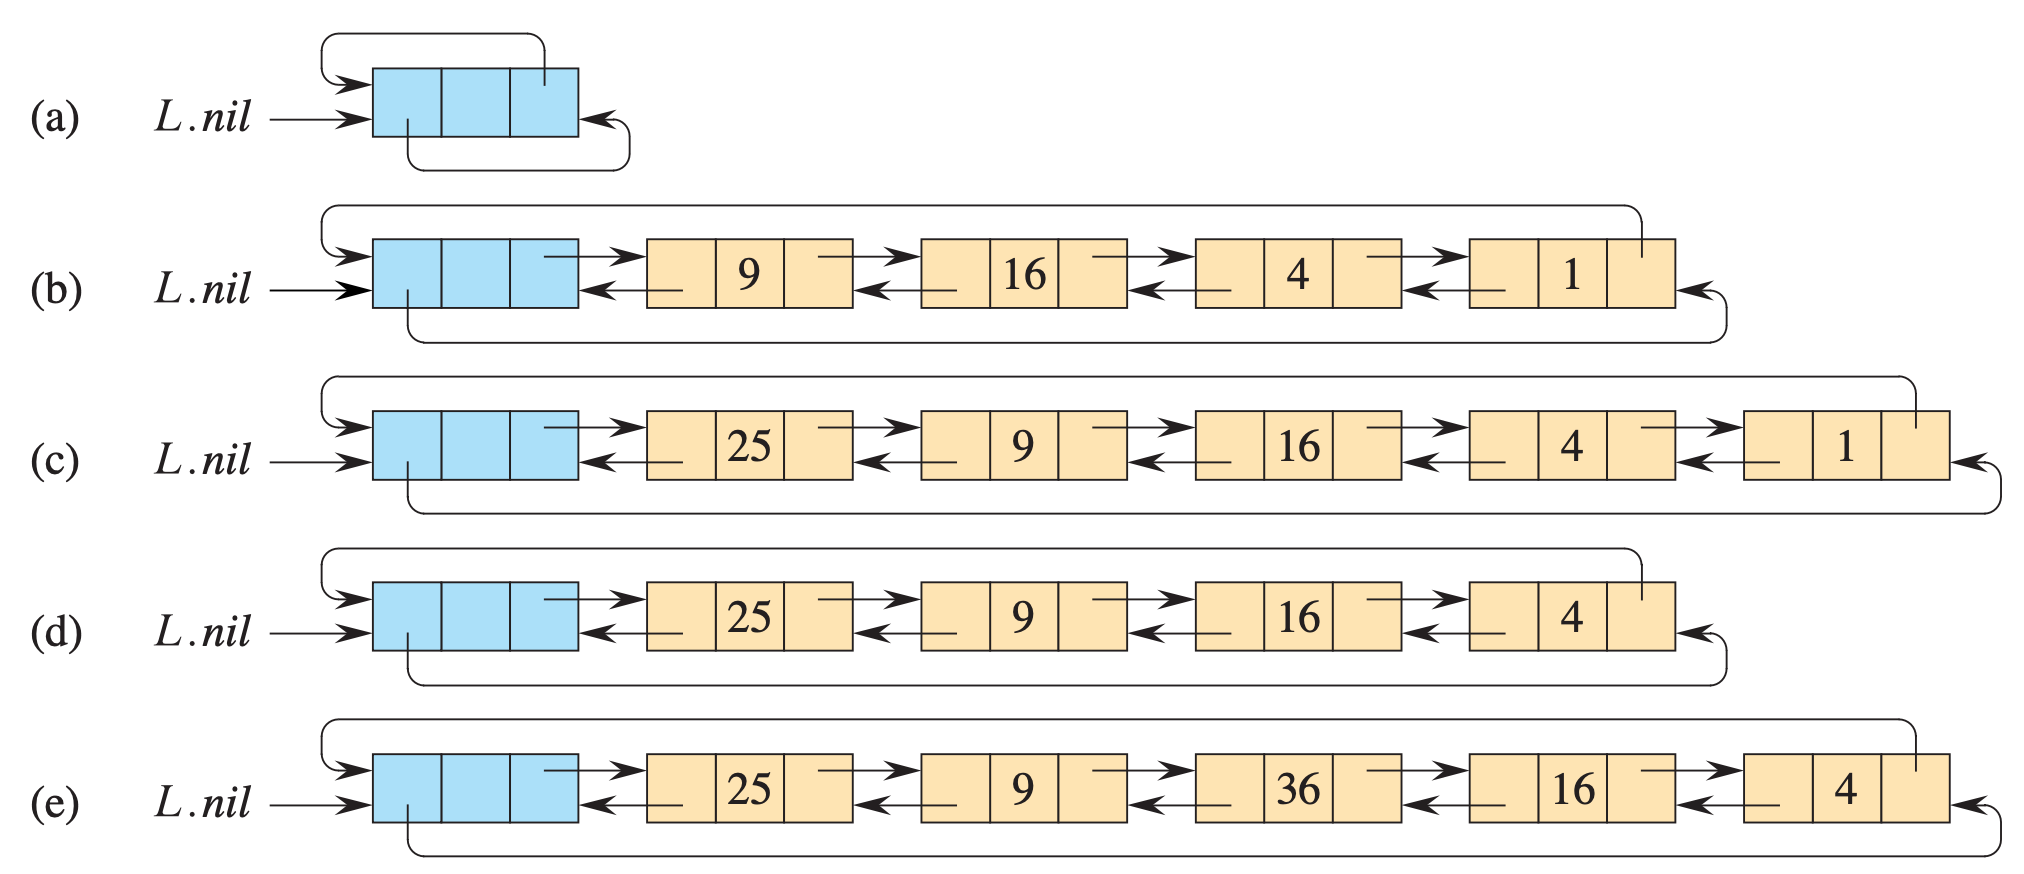
\includegraphics[width=0.7\textwidth]{./src/3.png}
\end{figure}

\subsection*{attempt}

\begin{enumerate}
\item
  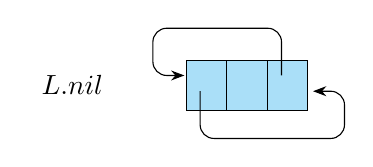
\begin{tikzpicture}[>=Stealth, start chain, node distance=10pt]
    \listNil
    \listHead{head}
    \draw[rounded corners=5pt,->]
    (head.one) -- ++ (0,-0.6)
    -- ($(head.three)+(0.8,-0.6)$)
    -- ++ (0,0.6)
    -- ++ (-0.4,0);
    \draw[rounded corners=5pt,->]
    ($(head.three)+(0,0.2)$) -- ++ (0,0.6)
    -- ($(head.one)+(-0.6,0.8)$)
    -- ++(0,-0.6)
    -- ++(0.4,0);
  \end{tikzpicture}
\item
  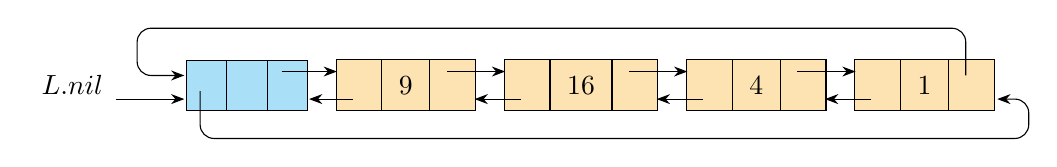
\begin{tikzpicture}[>=Stealth, start chain, node distance=10pt]
    \listNil
    \listHead{head}
    \foreach \Label in {9,16,4,1}
      \listNode{\Label}{$\Label$}
    ;

    \foreach \left/\right in {head/9, 9/16, 16/4, 4/1}{%
        \path[->] ($(\left.three)+(0,0.25)$) edge ($(\right.one)+(-0.2,0.25)$);%
        \path[->] ($(\right.one)+(0,-0.1)$) edge ($(\left.three)+(0.35,-0.1)$);%
    }
    \path[->] ($(nil.two)+(-0.2,-0.1)$) edge
    ($(head.one)+(-0.2,-0.1)$);%

    \draw[->, rounded corners=5pt] (head.one) -- ++ (0,-0.6)
    -- ($(1.three)+(0.8,-0.6)$) -- ($(1.three)+(0.8,-0.1)$)
    -- ($(1.three)+(0.4,-0.1)$);

    \draw[->, rounded corners=5pt]
    ($(1.three)+(0,0.2)$) -- ++ (0,0.6)
    -- ($(head.one)+(-0.8,0.8)$)
    -- ++(0,-0.6)
    -- ++(0.6,0);
  \end{tikzpicture}

\item
  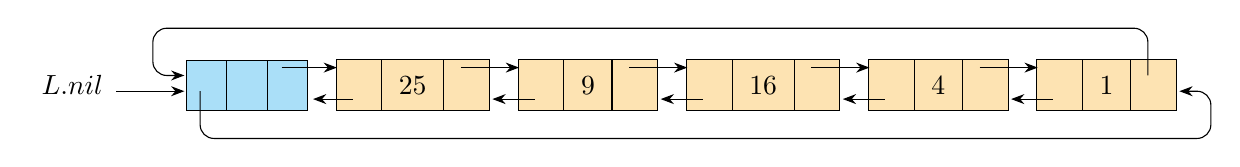
\begin{tikzpicture}[>=Stealth, node distance=10pt, start chain]
    \listNil
    \listHead{head}
    \foreach \Label in {25, 9, 16, 4, 1}{
      \listNode{\Label}{$\Label$}
    }
    \foreach \left/\right in {head/25, 25/9, 9/16, 16/4, 4/1}{
      \draw[->]
      ($(\left.three)+(0,0.3)$) -- ($(\right.one)+(-0.2,0.3)$);
      \draw[<-]
      ($(\left.three)+(0.4,-0.1)$) -- ($(\right.one)+(0,-0.1)$);
    }
    \draw[->, rounded corners=5pt]
    (head.one) -- ++ (0,-0.6)
    -- ($(1.three)+(0.8,-0.6)$)
    -- ++ (0,0.6)
    -- ++ (-0.4,0);
    \draw[->, rounded corners=5pt]
    ($(1.three)+(0,0.2)$)
    -- ++ (0,0.6)
    -- ($(head.one)+(-0.6,0.8)$)
    -- ++ (0,-0.6)
    -- ++ (0.4,0);
    \draw[->] ($(nil.two)+(-0.2,0)$) -- ($(head.one)+(-0.2,0)$);
  \end{tikzpicture}
\item
  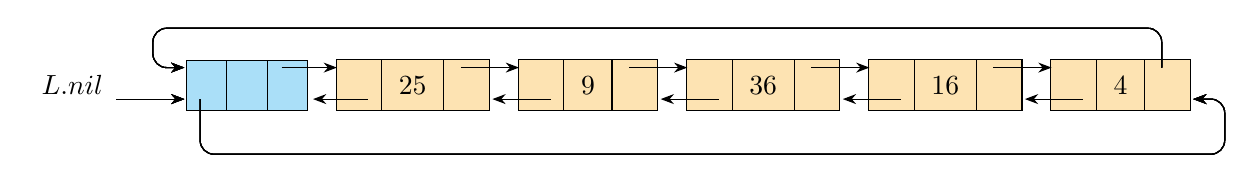
\begin{tikzpicture}[>=Stealth, node distance=10pt, start chain]
    \listNil
    \listHead{head}

    \foreach \Label in {25, 9, 36, 16, 4}{
      \listNode{\Label}{$\Label$}
    }

    \foreach \left/\right in {head/25, 25/9, 9/36, 36/16, 16/4}{
      \draw[->]
      ($(\left.three)+(0,0.3)$) -- ($(\right.one)+(-0.2,0.3)$);
      \draw[<-]
      ($(\left.three)+(0.4,-0.1)$) -- ($(\right.one)+(0.2,-0.1)$);
      \draw[->, rounded corners=5pt]
      ($(head.one)+(0,-0.1)$)
      -- ++ (0,-0.7)
      -- ($(4.three)+(0.8,-0.8)$)
      -- ++ (0,0.7)
      -- ++(-0.4,0);
      \draw[->, rounded corners=5pt]
      ($(4.three)+(0,0.3)$)
      -- ++ (0,0.5)
      -- ($(head.one)+(-0.6,0.8)$)
      -- ++ (0,-0.5)
      -- ++ (0.4,0);
      \draw[->]
      ($(nil.second)+(-0.2,-0.1)$) -- ($(head.one)+(-0.2,-0.1)$);
    }
  \end{tikzpicture}
\end{enumerate}

\pagebreak
\section{Picture-4}
\subsection*{Source}

\begin{figure}[h]
  \centering
  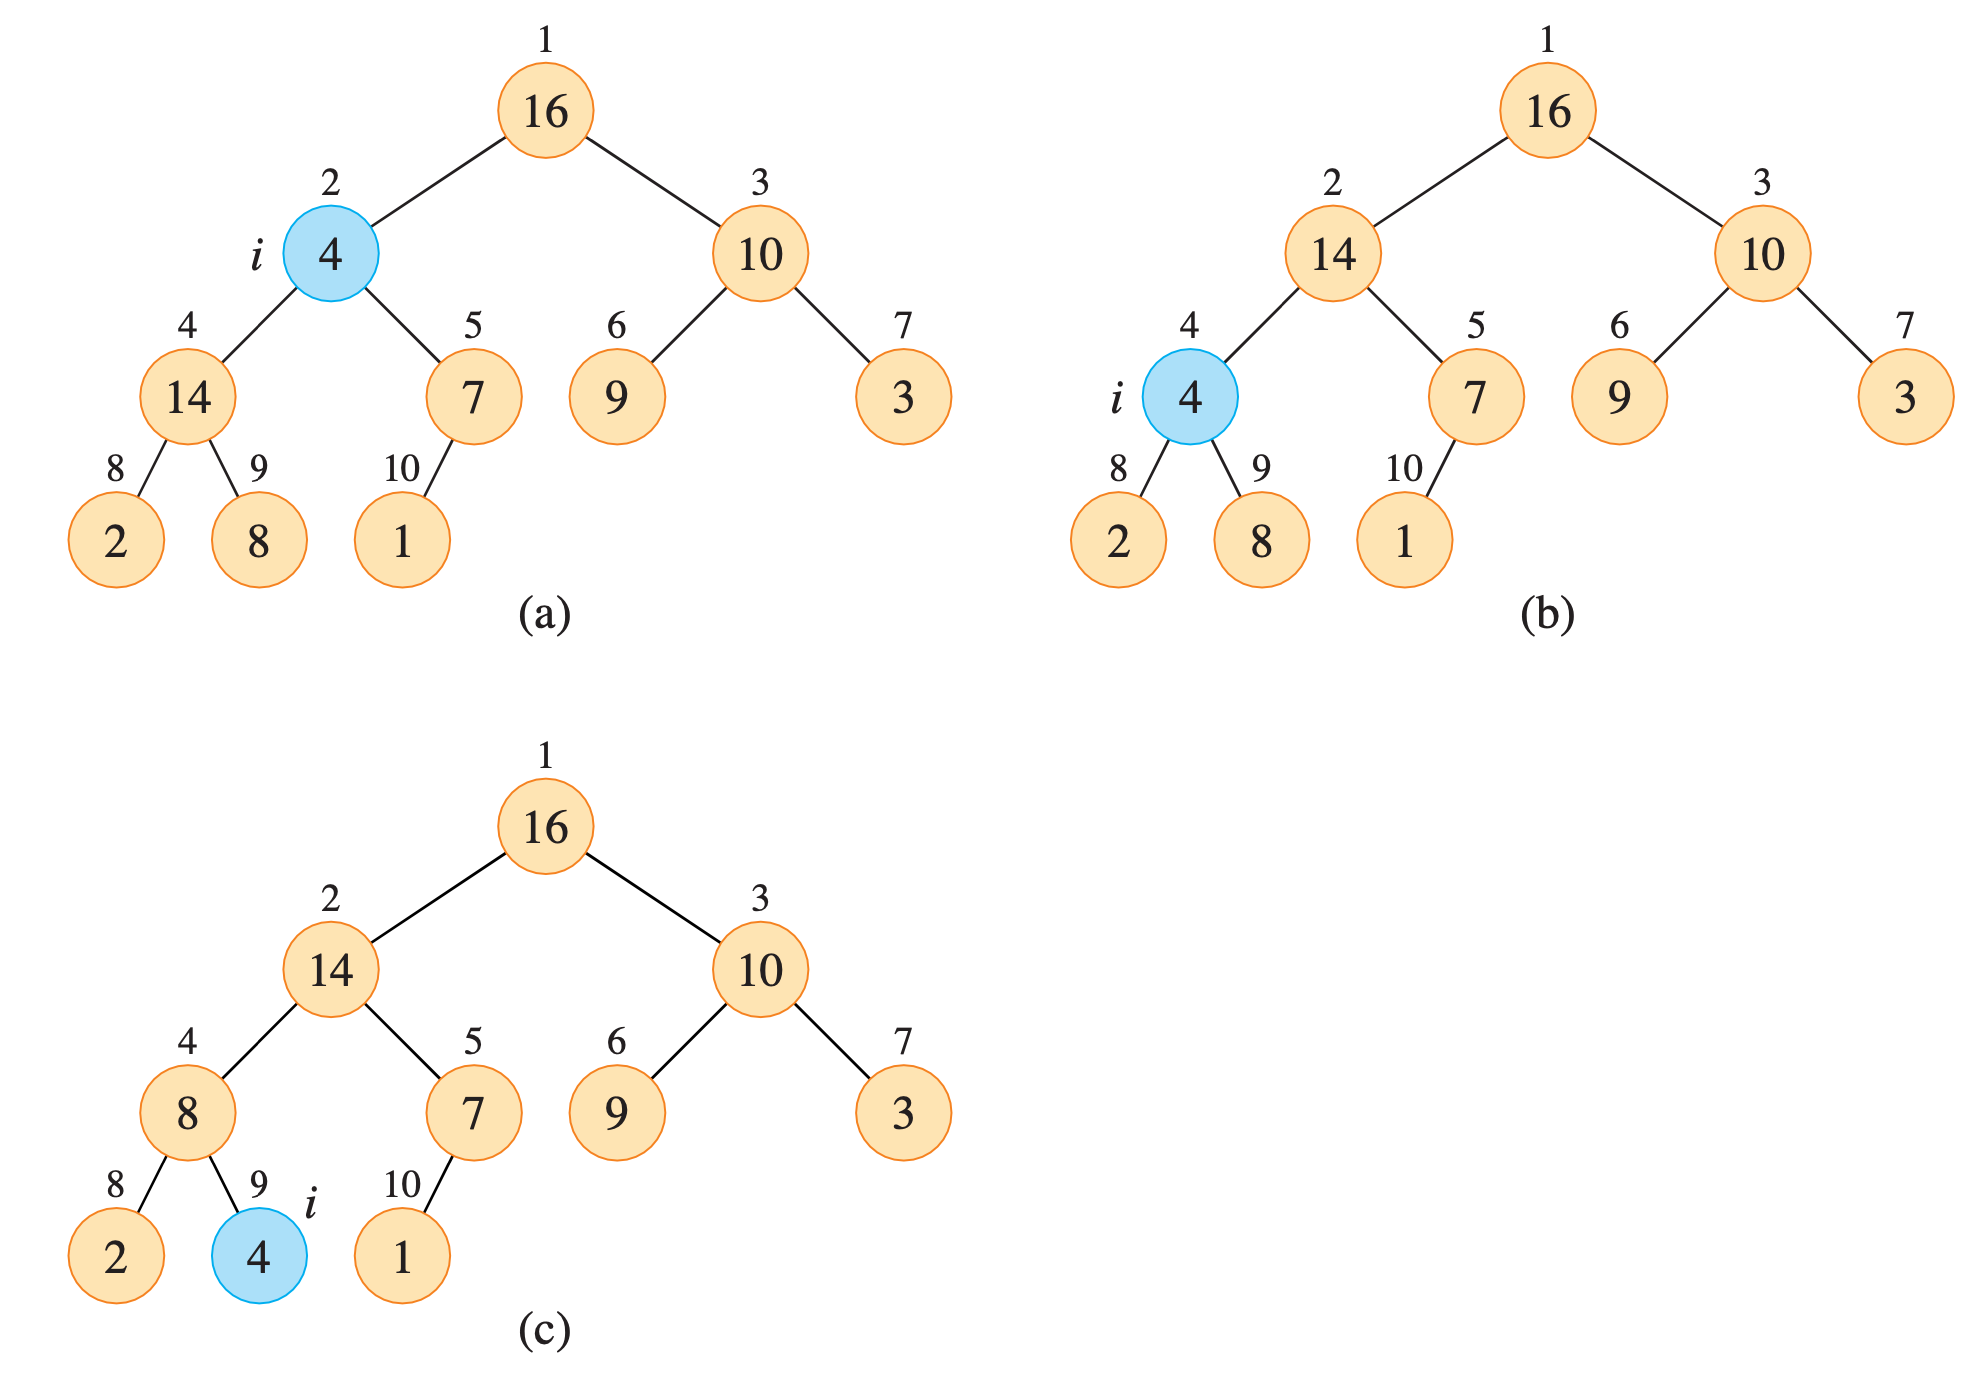
\includegraphics[width=0.7\textwidth]{./src/4.png}
\end{figure}

\subsection*{Attempt}

\newcommand{\scale}{0.6}
\begin{figure}[h]
  \begin{subfigure}[t]{0.5\textwidth}\vskip 0pt
    \begin{tikzpicture}[%
      scale=\scale,
      level distance=1.75cm,
      sibling distance=1.75cm,
      nodes={
        draw,
        circle,
        color=darkOrange,
        fill=lightOrange,
        text=black,
        inner sep=3pt,
        outer sep=0pt,
        minimum size=3ex
      }
      ]
      
      \tikzset{
        blueNode/.style={
          color=darkBlue,
          fill=skyBlue,
          text=black
        }
      }
      
      % 1 - inner label
      % 2 - outer label
      % 3 - i pos
      \newcommand{\NodeRoot}[2]{\node[label=above:#2]{#1}}
      \newcommand{\Node}[2]{node[label=above:#2]{#1}}
      \newcommand{\NodeBlue}[3]{%
        node[blueNode,label=above:#2,label=#3:$i$]{#1}%
      } 
      
      \NodeRoot{16}{1}
      child {\NodeBlue{4}{2}{left}
        child {\Node{14}{4}
          child {\Node{2}{8}}
          child {\Node{8}{9}}
        }
        child[missing]
        child {\Node{7}{5}
          child {\Node{1}{10}}
          child[missing]
        }
      }
      child[missing]
      child[missing]
      child {\Node{10}{3}
        child {\Node{9}{6}}
        child[missing]
        child {\Node{3}{7}}
      };
    \end{tikzpicture}
    \caption{~}
  \end{subfigure}\hfill\begin{subfigure}[t]{0.5\textwidth}\vskip 0pt
    \begin{tikzpicture}[%
      scale=\scale,
      level distance=1.75cm,
      sibling distance=1.75cm,
      nodes={
        draw,
        circle,
        color=darkOrange,
        fill=lightOrange,
        text=black,
        inner sep=3pt,
        outer sep=0pt,
        minimum size=3ex
      }
      ]
      
      \tikzset{
        blueNode/.style={
          color=darkBlue,
          fill=skyBlue,
          text=black
        }
      }
      
      % 1 - inner label
      % 2 - outer label
      % 3 - i pos
      \newcommand{\NodeRoot}[2]{\node[label=above:#2]{#1}}
      \newcommand{\Node}[2]{node[label=above:#2]{#1}}
      \newcommand{\NodeBlue}[3]{%
        node[blueNode,label=above:#2,label=#3:$i$]{#1}%
      } 
      
      \NodeRoot{16}{1}
      child {\Node{14}{2}
        child {\NodeBlue{4}{2}{left}
          child {\Node{2}{8}}
          child {\Node{8}{9}}
        }
        child[missing]
        child {\Node{7}{5}
          child {\Node{1}{10}}
          child[missing]
        }
      }
      child[missing]
      child[missing]
      child {\Node{10}{3}
        child {\Node{9}{6}}
        child[missing]
        child {\Node{3}{7}}
      };
    \end{tikzpicture}
    \caption{~}
  \end{subfigure}

  \begin{subfigure}[t]{0.5\textwidth}\vskip 0pt
    \begin{tikzpicture}[%
      scale=\scale,
      level distance=1.75cm,
      sibling distance=1.75cm,
      nodes={
        draw,
        circle,
        color=darkOrange,
        fill=lightOrange,
        text=black,
        inner sep=3pt,
        outer sep=0pt,
        minimum size=3ex
      }
      ]
      
      \tikzset{
        blueNode/.style={
          color=darkBlue,
          fill=skyBlue,
          text=black
        }
      }
      
      % 1 - inner label
      % 2 - outer label
      % 3 - i pos
      \newcommand{\NodeRoot}[2]{\node[label=above:#2]{#1}}
      \newcommand{\Node}[2]{node[label=above:#2]{#1}}
      \newcommand{\NodeBlue}[3]{%
        node[blueNode,label=above:#2,label=#3:$i$]{#1}%
      } 
      
      \NodeRoot{16}{1}
      child {\Node{14}{2}
        child {\Node{8}{2}
          child {\Node{2}{8}}
          child {\NodeBlue{4}{9}{above right}}
        }
        child[missing]
        child {\Node{7}{5}
          child {\Node{1}{10}}
          child[missing]
        }
      }
      child[missing]
      child[missing]
      child {\Node{10}{3}
        child {\Node{9}{6}}
        child[missing]
        child {\Node{3}{7}}
      };
    \end{tikzpicture}
    \caption{~}
  \end{subfigure}
\end{figure}

\pagebreak
\section{Picture-5}
\subsection*{Source}
\begin{figure}[h]
  \centering
  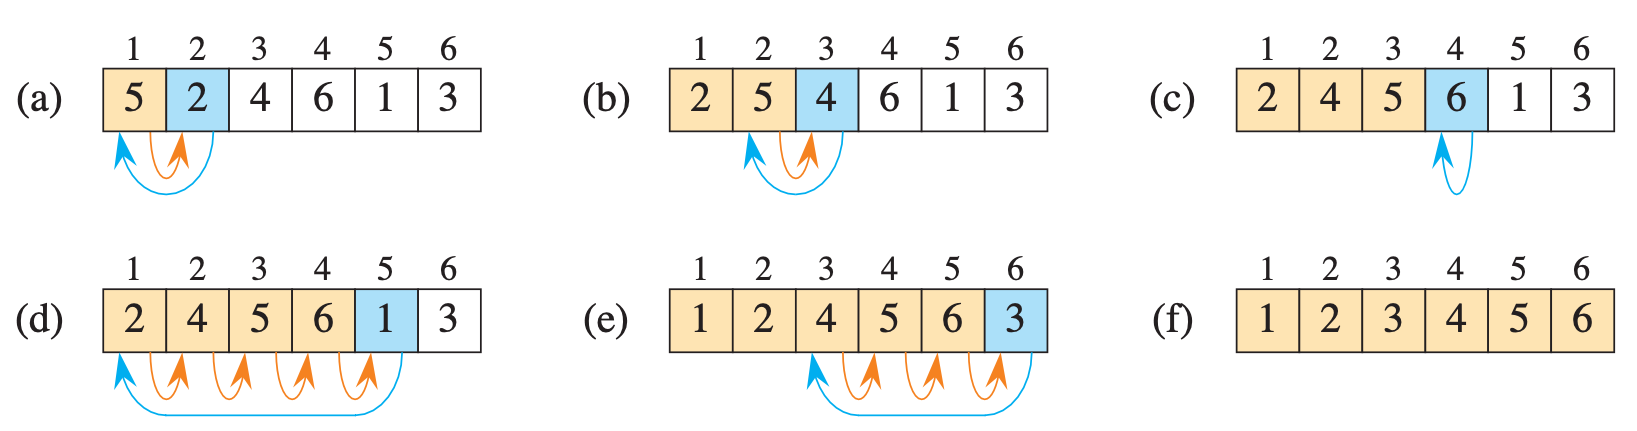
\includegraphics[width=\textwidth]{./src/5.png}
\end{figure}

\subsection*{Attempt}
\begin{figure}[h]
  \begin{subfigure}[T]{0.3\textwidth}\vskip 0pt
    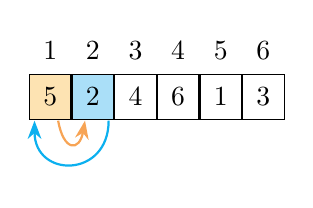
\begin{tikzpicture}[
      >=Stealth,
      every node/.style={
        inner sep=5pt,
        anchor=south,
        draw
      },
      node distance=0pt,
      start chain
      ]
      
      \node[on chain,label=above:1, fill=lightOrange] (1) {5};
      \node[on chain,label=above:2, fill=skyBlue] (2) {2};

      \foreach \i/\j in {3/4, 4/6, 5/1, 6/3}{
        \node[on chain, label=above:\i] (\i) {\j};
      }
      
      \draw[->, looseness=2, thick, color=darkBlue]
      ($(2)+(0.2,-0.3)$) to[out=270, in=270] ($(1)+(-0.2,-0.3)$);
      
      \draw[->, looseness=3, thick, color=darkOrange]
      ($(1)+(0.1,-0.3)$) to[out=280,in=260] ($(2)+(-0.1,-0.3)$);
    \end{tikzpicture}
    \caption{~}
  \end{subfigure}\hfill\begin{subfigure}[T]{0.3\textwidth}\vskip 0pt
    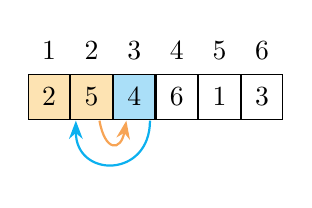
\begin{tikzpicture}[
      >=Stealth,
      every node/.style={
      inner sep=5pt,
      anchor=south,
      draw
    },
      node distance=0pt,
      start chain
      ]

      \node[on chain,label=above:1, fill=lightOrange] (1) {2};
      \node[on chain,label=above:2, fill=lightOrange] (2) {5};
      \node[on chain,label=above:3, fill=skyBlue] (3) {4};

      \foreach \i/\j in {4/6, 5/1, 6/3}{
        \node[on chain, label=above:\i] (\i) {\j};
      }
      
      \draw[->, looseness=2, thick, color=darkBlue]
      ($(3)+(0.2,-0.3)$) to[out=270, in=270] ($(2)+(-0.2,-0.3)$);
    
      \draw[->, looseness=3, thick, color=darkOrange]
      ($(2)+(0.1,-0.3)$) to[out=280,in=260] ($(3)+(-0.1,-0.3)$);
    \end{tikzpicture}
    \caption{~}
  \end{subfigure}\hfill\begin{subfigure}[T]{0.3\textwidth}\vskip 0pt
    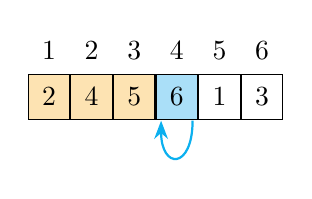
\begin{tikzpicture}[
      >=Stealth,
      every node/.style={
        inner sep=5pt,
        anchor=south,
        draw
      },
      node distance=0pt,
      start chain
      ]

      \foreach \i/\j in {1/2, 2/4, 3/5}{
        \node[on chain,label=above:\i, fill=lightOrange] (\i) {\j};
      }

      \node[on chain,label=above:4, fill=skyBlue] (4) {6};
      \node[on chain,label=above:5] (5) {1};
      \node[on chain,label=above:6] (6) {3};
      
      \draw[->, looseness=4, color=darkBlue, thick]
      ($(4)+(0.2,-0.3)$) to[out=270, in=270] ($(4)+(-0.2,-0.3)$);
    \end{tikzpicture}
    \caption{~}
  \end{subfigure}

  \begin{subfigure}[T]{0.3\textwidth}\vskip 0pt
    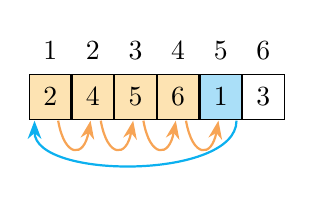
\begin{tikzpicture}[
      >=Stealth,
      every node/.style={
        inner sep=5pt,
        anchor=south,
        draw
      },
      node distance=0pt,
      start chain
      ]

      \foreach \i/\j in {1/2, 2/4, 3/5, 4/6}{
        \node[on chain,label=above:\i, fill=lightOrange] (\i) {\j};
      }
     \node[on chain,label=above:5, fill=skyBlue] (5) {1};
      \node[on chain,label=above:6] (6) {3};
      
      \foreach \i in {1,...,4}{
        \tikzmath{
          \j=\i+1;
        }
        \draw[->, looseness=3, thick, color=darkOrange]
        ($(\i)+(0.1,-0.3)$) to[out=280,in=260] ($(\j)+(-0.3,-0.3)$);
      }
      
      \draw[->, looseness=0.75, color=darkBlue, thick]
      ($(5)+(0.2,-0.3)$) to[out=270, in=270] ($(1)+(-0.2,-0.3)$);
    \end{tikzpicture}
    \caption{~}
  \end{subfigure}\hfill\begin{subfigure}[T]{0.3\textwidth}\vskip 0pt
    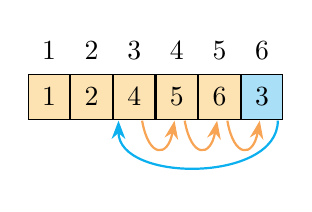
\begin{tikzpicture}[
      >=Stealth,
      every node/.style={
        inner sep=5pt,
        anchor=south,
        draw
      },
      node distance=0pt,
      start chain
      ]

      \foreach \i/\j in {1/1, 2/2, 3/4, 4/5, 5/6}{
        \node[on chain,label=above:\i, fill=lightOrange] (\i) {\j};
      }
      \node[on chain,label=above:6, fill=skyBlue] (6) {3};
      
      \foreach \i in {3,...,5}{
        \tikzmath{
          \j=\i+1;
        }
        \draw[->, looseness=3, thick, color=darkOrange]
        ($(\i)+(0.1,-0.3)$) to[out=280,in=260] ($(\j)+(-0.3,-0.3)$);
      }
      \draw[->, looseness=1, color=darkBlue, thick]
      ($(6)+(0.2,-0.3)$) to[out=270, in=270] ($(3)+(-0.2,-0.3)$);
    \end{tikzpicture}
    \caption{~}
  \end{subfigure}\hfill\begin{subfigure}[T]{0.3\textwidth}\vskip 0pt
    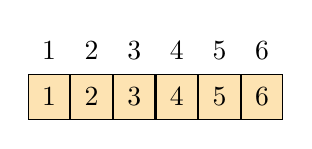
\begin{tikzpicture}[
      >=Stealth,
      every node/.style={
        inner sep=5pt,
        anchor=south,
        draw
      },
      node distance=0pt,
      start chain
      ]
      
      \foreach \i in {1,...,6}{
        \node[on chain,label=above:\i, fill=lightOrange] (\i) {\i};
      }
    \end{tikzpicture}
    \caption{~}
  \end{subfigure}
\end{figure}

\pagebreak
\section{Picture-6}
\subsection*{Source}
\begin{figure}[h]
  \centering
  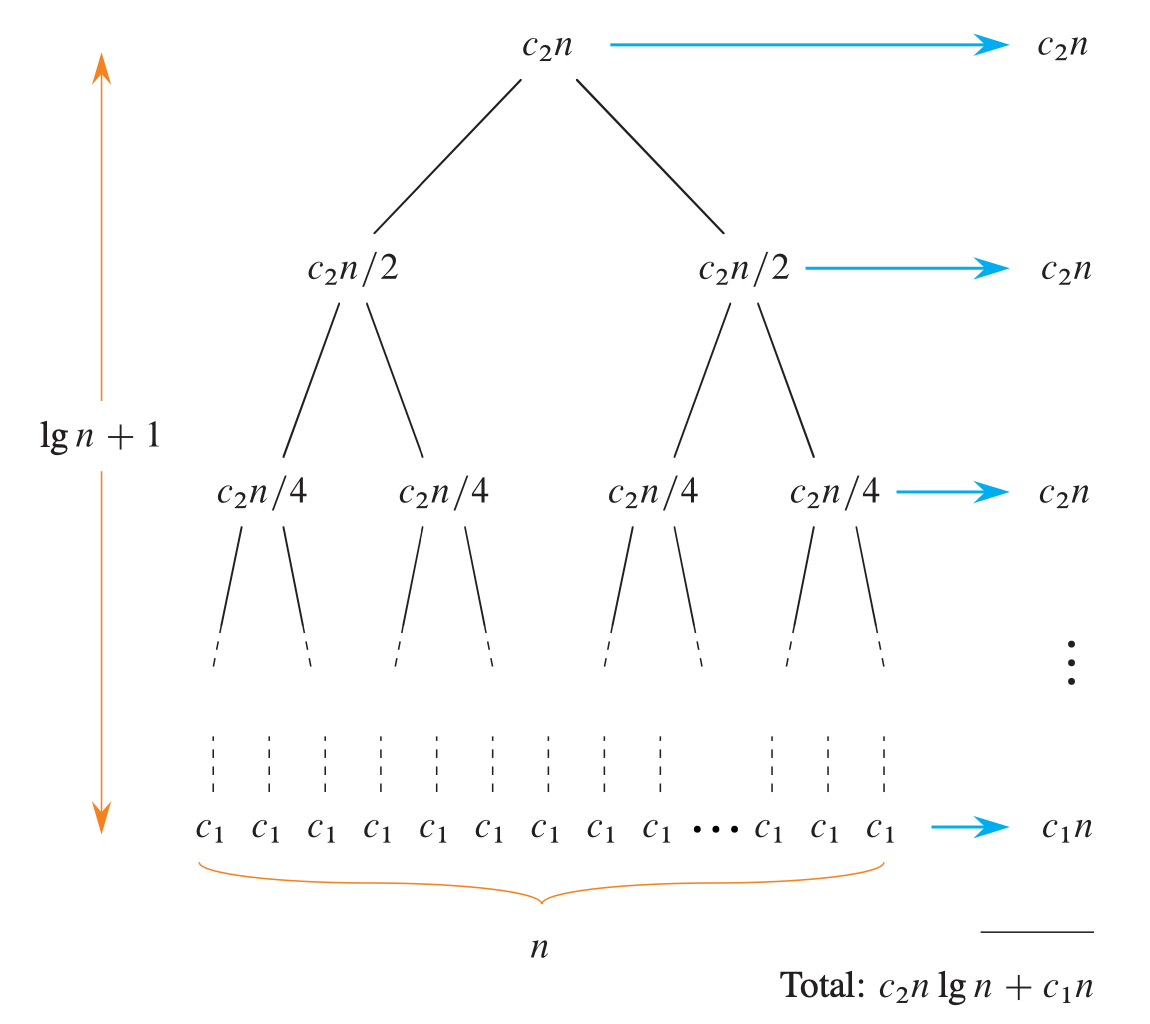
\includegraphics[width=1\textwidth]{./src/6.png}
\end{figure}

\pagebreak
\subsection*{Attempt}

\begin{figure}[h]
  \centering
  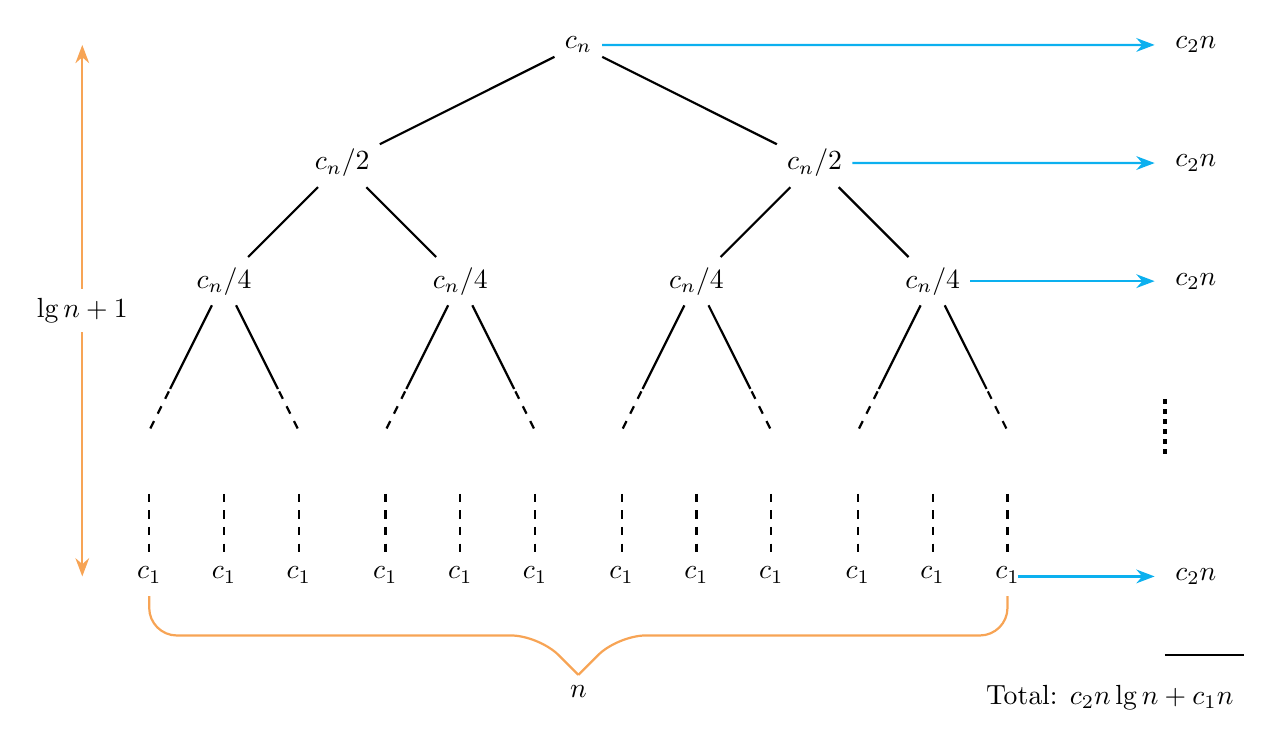
\begin{tikzpicture}[thick, >=Stealth]
    \node (right1) {$c_n$}
    child{ node{$c_n/2$}
      child{node (last1) {$c_n/4$}
        child{node (leaf1) {~}}
        child{node (leaf2) {~}}
      }
      child[missing]
      child{node (last2) {$c_n/4$}
        child{node (leaf3) {~}}
        child{node (leaf4) {~}}
      }
    }
    child[missing]
    child[missing]
    child[missing]
    child{ node (right2) {$c_n/2$}
      child{node (last3) {$c_n/4$}
        child{node (leaf5) {~}}
        child{node (leaf6) {~}}
      }
      child[missing]
      child{node (right3) {$c_n/4$}
        child{node (leaf7) {~}}
        child{node (leaf8) {~}}
      }
    }
    ;

    \foreach \i in {1,3,...,8}{
      \draw[dashed] ($(leaf\i)+(0.05,0.1)$) --
      ($(leaf\i)+(-0.2,-0.4)$);
    }

    \foreach \i in {2,4,...,8}{
      \draw[dashed] ($(leaf\i)+(-0.05,0.1)$) --
      ($(leaf\i)+(0.2,-0.4)$);
    }

    \foreach \i in {1,3,...,8}{
      \draw[dashed] 
      ($(leaf\i)+(-0.2,-1.2)$) --
      ($(leaf\i)+(-0.2,-2)$)
      node [below] {$c_1$}
      ;
    }

    \foreach \i in {2,4,...,8}{
      \draw[dashed] 
      ($(leaf\i)+(0.2,-1.2)$) --
      ($(leaf\i)+(0.2,-2)$)
      node [below] {$c_1$}
      ;
    }

    \draw[dashed]
    ($(right3)+(0,-2.7)$) -- ($(right3)+(0,-3.5)$)
    node [below] {$c_1$}
    ;

    \foreach \i in {1,...,3}{
      \draw[dashed]
      ($(last\i)+(0,-2.7)$) -- ($(last\i)+(0,-3.5)$)
      node [below] {$c_1$};
    }

    \node (right4) at ($(leaf8)+(0.2,-2.25)$) {};

    \node (level4) at ($(right4)+(2,0)$)      {};
    \node (level3) at ($(level4)+(0,3.75)$)    {};
    \node (level2) at ($(level3)+(0,1.5)$)   {};
    \node (level1) at ($(level2)+(0,1.5)$)   {};

    \foreach \i in {1,...,4}{
      \draw[->,thick,darkBlue]
      (right\i) -- (level\i)
      node[right,text=black] {$c_2n$}
      ;
    }

    \draw[dotted, ultra thick]
    ($(level3)+(0,-1.5)$) --
    ($(level4)+(0,1.5)$);

    \draw
    ($(level4)+(0,-1)$) --
    ($(level4)+(1,-1)$);

    \node at ($(level4)+(1,-1.25)$) [below left] {Total: $c_2n\lg
      n+c_1n$};

    \draw[rounded corners=10pt, thick, darkOrange]
    ($(leaf1)!0.5!(leaf8) + (0,-3.5)$)
    -- ++ (-0.5,0.5)
    --
    ($(leaf1)+(-0.2,-3)$)
    --
    ($(leaf1)+(-0.2,-2.5)$)
    ;
    \draw[rounded corners=10pt, thick, darkOrange]
    ($(leaf1)!0.5!(leaf8) + (0,-3.5)$)
    -- ++ (0.5,0.5)
    --
    ($(leaf8)+(0.2,-3)$)
    --
    ($(leaf8)+(0.2,-2.5)$)
    ;
    \node at ($(leaf1)!0.5!(leaf8) + (0,-3.5)$) [below] {$n$};

    \draw[<->, darkOrange]
    ($(level1)+(-13.75,0)$)
    --
    node[midway,fill=white,text=black] {$\lg n+1$}
    ($(level4)+(-13.75,0)$)
    ;
 \end{tikzpicture}
\end{figure}
\end{document}
